\subsection*{Subscription queries} % (fold)
\label{sub:Subscription business queries}
If the row number is not explicitly specified than full results are presented.
\begin{enumerate}
  \item Revenue from subscriptions by year?
\begin{lstlisting}[language=sql]
select sum(price * (1-discount) * quantity) revenue, d.year 
from sub_subscription s 
join sub_date d on s.keydate = d.keydate 
group by d.year 
order by year desc;
\end{lstlisting}
    2.444s \\ \\
      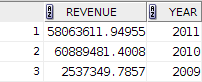
\includegraphics[scale=0.5]{sub_1}
  \item Which were the most popular subscription periods each year?
\begin{lstlisting}[language=sql]
select year, p.name as period, sum(quantity) subscriptions
from oplatek.sub_subscription s 
join oplatek.sub_date d on s.keydate = d.keydate
join oplatek.sub_period p on s.keyperiod = p.keyperiod 
group by d.year, p.name
order by year desc, subscriptions desc;
\end{lstlisting}
    0.808s \\ \\
      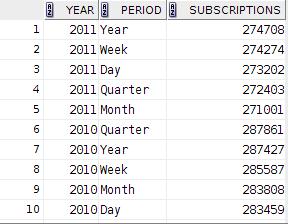
\includegraphics[scale=0.5]{sub_2}
  \item Revenue from subscriptions and subscription count by country in 2010?
\begin{lstlisting}[language=sql]
select l.country, sum(price * (1-discount) * quantity) revenue, 
  sum(quantity) subscriptions 
from oplatek.sub_subscription s 
join oplatek.sub_location l on s.keylocation = l.keylocation 
join oplatek.sub_date d on s.keydate=d.keydate and d.year=2010
group by l.country 
order by revenue desc;
\end{lstlisting}
     0.639s \\ \\
      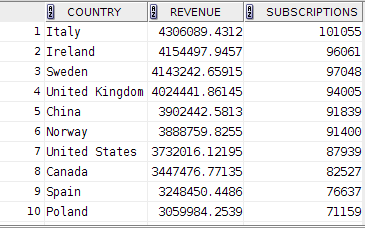
\includegraphics[scale=0.5]{sub_3}
  \item Top 10 cities from each country with the highest revenue from subscriptions in 2010?
\begin{lstlisting}[language=sql]  
select * from (select country, city, 
  sum(price * (1-discount) * quantity) revenue, 
  rank() over(partition by country 
    order by sum(price * (1-discount) * quantity) desc) rank 
from oplatek.sub_subscription s 
join oplatek.sub_date d 
  on s.keydate = d.keydate and d.year = 2010
join oplatek.sub_location l 
  on s.keylocation = l.keylocation
group by l.country, l.city
order by revenue desc)
where rank <= 10;
\end{lstlisting}
     50 rows 0.711s\\ \\
      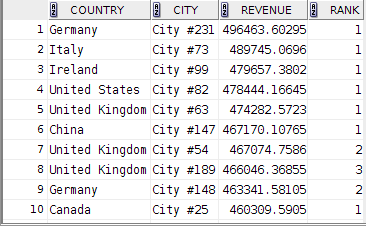
\includegraphics[scale=0.5]{sub_4}
  \item How much would we earn without applying discounts on subscriptions, by period type and by year?
\begin{lstlisting}[language=sql] 
select year, period, revenue, revenue_no_discounts, 
  (revenue_no_discounts - revenue) difference from 
    (select d.year, p.name as period, 
      sum(price * (1-discount) * quantity) revenue, 
      sum(price * quantity) revenue_no_discounts
     from oplatek.sub_subscription s 
     join oplatek.sub_date d on s.keydate = d.keydate
     join oplatek.sub_period p on s.keyperiod = p.keyperiod
     group by d.year, p.name)
order by year desc, period asc;
\end{lstlisting}
     1.127s \\ \\
      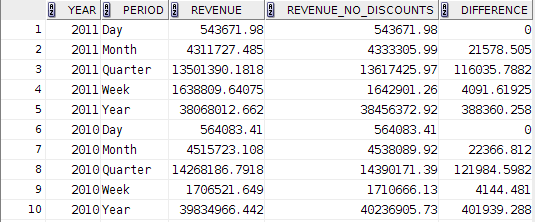
\includegraphics[scale=0.5]{sub_5}
%  \item Comparison of the number of sales on Christmas and Easter by period in Canada in 2010?
%\begin{lstlisting}[language=sql] 
%select sum(quantity) from 
%    oplatek.sub_subscription ss, oplatek.sub_date dd 
% where ss.keydate = dd.keydate and dd.Easter = 'Y' 
%  and ss.keyperiod = p.keyperiod 
%  and ss.keylocation = l.keylocation as easter,
%select country, year, period, total_sales, 
% from (select l.country, d.year, 
%         p.name period, sum(quantity) total_sales
%       from oplatek.sub_subscription s 
%       join oplatek.sub_date d 
%         on s.keydate = d.keydate and d.year = 2010
%       join oplatek.sub_location l 
%         on s.keylocation = l.keylocation 
%         and l.country = 'Canada'
%       join oplatek.sub_period p on s.keyperiod = p.keyperiod 
%       group by l.country, d.year, p.name)
%order by d.year, period;
%\end{lstlisting}
%     todo s \\ \\
%      \includegraphics[scale=0.5]{sub_6}
  \item[7.] Revenue by month and by state in Canada in 2010 together with average revenue by states in Canada in the same month?
\begin{lstlisting}[language=sql] 
select l.state, d.month, 
  sum(price * (1-discount) * quantity) revenue,
  /* avg_revenue_in_this_month_across_all_states */
  avg(sum(price * (1-discount) * quantity)) 
    over (partition by month) avg_rev 
from oplatek.sub_subscription s 
join oplatek.sub_location l 
    on s.keylocation = l.keylocation and l.country = 'Canada' 
join oplatek.sub_date d 
    on s.keydate = d.keydate and d.year = 2010
where length(l.state) = 2
group by l.state, d.month
order by state asc, month asc;
\end{lstlisting}
      156 rows 0.711s\\ \\
      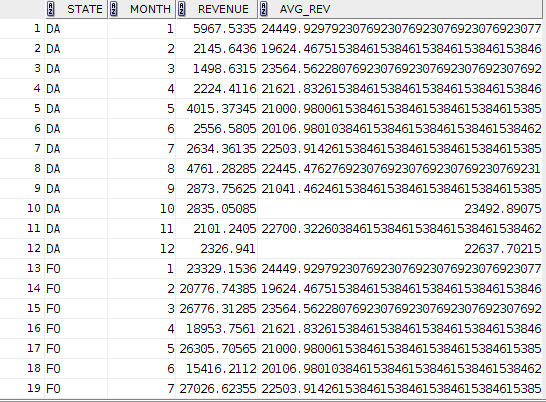
\includegraphics[scale=0.5]{sub_7}
\end{enumerate}
% subsection Subscription queries (end)

\subsection*{Article queries} % (fold)
\label{sub:Article  queries}
\begin{enumerate}
\item    Top 10 read articles and their authors for every month in year 2011?
\begin{lstlisting}[language=sql] 
select * from (
 select d.month, a.keyarticle as id, 
  a.title, a.author, sum(reads) reads, 
  rank() over (partition by month order by sum(reads) desc) rank 
 from oplatek.artpop_articlepopularity f
 join oplatek.artpop_article a on f.keyarticle = a.keyarticle
 join oplatek.artpop_date d on f.keydate = d.keydate 
     and d.year = 2010
 group by d.month, a.keyarticle, a.title, a.author
 order by month asc, reads desc
) where rank <= 10;
\end{lstlisting}
     121 rows 2.604s \\ \\
      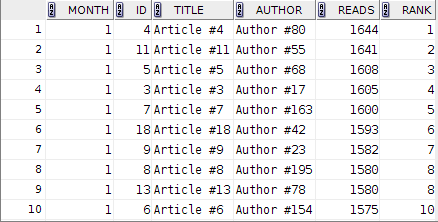
\includegraphics[scale=0.5]{art_1}
\item    Hours of the day when most articles are read grouped by category in year 2010 together with the average number of articles read during this hour in the same year?
\begin{lstlisting}[language=sql] 
select a.category, d.hour, sum(reads) reads, 
    avg(sum(reads)) over (partition by hour) avg_reads 
from oplatek.artpop_articlepopularity f
join oplatek.artpop_article a on f.keyarticle = a.keyarticle
join oplatek.artpop_date d on f.keydate = d.keydate 
    and d.year = 2010
group by a.category, d.hour
order by a.category asc, d.hour asc;
\end{lstlisting}
     96 rows 0.415s \\ \\
      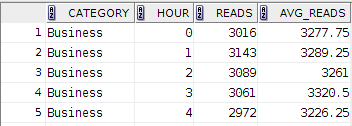
\includegraphics[scale=0.5]{art_2}
\item    Number of articles published in each subcategory in year 2010 together with the percentage of total articles in the category?
\begin{lstlisting}[language=sql] 
select category, subcategory, 
 articles/sum(articles) over (partition by category) perct, 
 articles, 
 sum(articles) over (partition by category) as articles_in_category 
 from (
  select a.category, a.subcategory, count(a.keyarticle) articles
  from oplatek.artpop_articlepopularity f
  join oplatek.artpop_article a 
   on f.keyarticle = a.keyarticle and a.publicationyear = 2011
  group by a.category, a.subcategory
  order by category, subcategory
 );
\end{lstlisting}
     1.23s\\ \\
      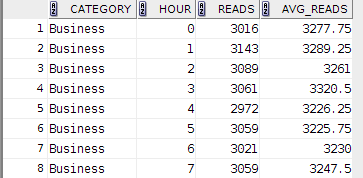
\includegraphics[scale=0.5]{art_3}
\item    Top 5 authors in every category by comments on their articles?
\begin{lstlisting}[language=sql] 
select * from (
select a.category, a.author, sum(comments) comments, 
  rank() over (partition by a.category 
    order by sum(comments) desc) rank 
from oplatek.artpop_articlepopularity f
join oplatek.artpop_article a on f.keyarticle = a.keyarticle
group by a.category, a.author
order by a.category asc, comments desc
) where rank <= 5;
\end{lstlisting}
     0.823 s\\ \\
      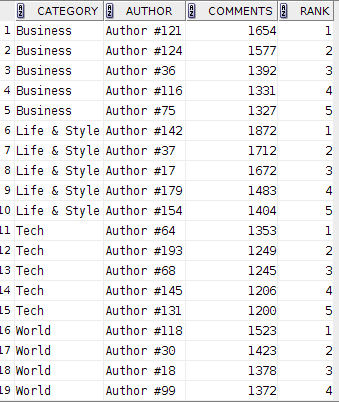
\includegraphics[scale=0.5]{art_4}
%\item    Each author's 5 most read articles with the number of total article reads together with the average number of article reads for this author's department and each author must have at least 20 articles published, all these articles must have been published before 2011 and total reads for each article must be above the average article read count for the author's department?
%\begin{lstlisting}[language=sql] 
%select *
%from (select a.author, 
%  rank() 
%    over (partition by a.author order by sum(reads) desc) rank,
%  a.keyarticle id, a.title,
%  sum(reads) reads, 
%  a.authordepartment department,
%  avg(sum(reads)) 
%    over (partition by a.authordepartment) deparment_reads,
%  count(a.keyarticle) 
%    over (partition by a.author) total_articles
%from oplatek.artpop_articlepopularity f
%join oplatek.artpop_article a on f.keyarticle = a.keyarticle
%where a.publicationyear < 2011
%group by a.author, a.authordepartment, a.keyarticle, a.title
%order by a.author, rank asc)
%where rank <= 5 and reads > deparment_reads 
%and total_articles >= 20;
%\end{lstlisting}
%     todo  !!s \\ \\
%      \includegraphics[scale=0.5]{art_5}
\item    Top 20 articles published in October, 2011 with the \#comments/\#reads higher than the average \#comments/\#reads having at least 20000 \#reads?
\begin{lstlisting}[language=sql] 
select * from (
select a.keyarticle id, a.title,
   sum(reads)/sum(comments) comm_by_reads,
   avg(sum(reads)/sum(comments)) over () avg_comm_by_reads,
   sum(reads) reads
from oplatek.artpop_articlepopularity f
join oplatek.artpop_article a on f.keyarticle = a.keyarticle
where a.publicationyear = 2011 
and a.publicationmonth = 10
group by a.keyarticle, a.title
order by comm_by_reads - avg_comm_by_reads desc
) where comm_by_reads > avg_comm_by_reads 
and reads >= 20000 and rownum <= 20;
\end{lstlisting}
     1.125 s\\ \\
      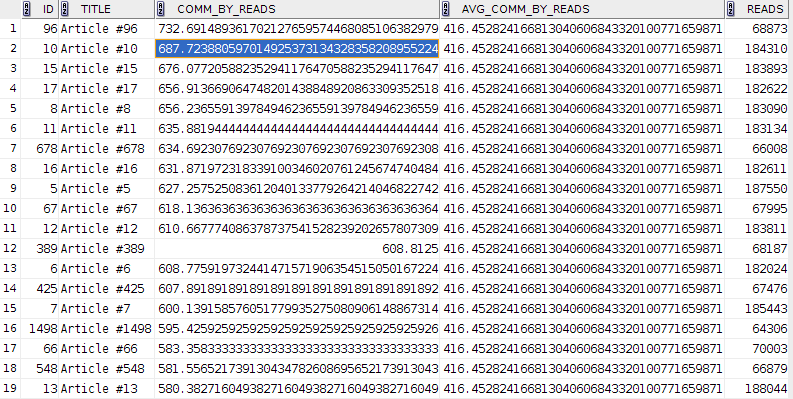
\includegraphics[scale=0.5]{art_6}
\item    Compare the number of reads/shares/comments of articles tagged with tags 'positive' and 'negative' for each year?
\begin{lstlisting}[language=sql] 
select year, tag, reads, 
 sum(reads) over (partition by year) reads_total, 
 reads/sum(reads) over (partition by year) reads_perc,
 reads, sum(shares) over (partition by year) shares_total, 
 shares/sum(shares) over (partition by year) shares_perc,
 reads, sum(comments) over (partition by year) comments_total, 
 comments/sum(comments) over (partition by year) comments_perc
from (
 select a.publicationyear year, t.tag, sum(reads) reads, 
  sum(comments) comments, sum(shares) shares
 from oplatek.artpop_articlepopularity f
 join oplatek.artpop_article a on f.keyarticle = a.keyarticle
 join oplatek.artpop_tag t on t.tag in ('positive', 'negative')
 join oplatek.artpop_articletags artt 
  on a.keyarticle = artt.keyarticle and artt.keytag = t.keytag 
 group by a.publicationyear, t.tag
 order by year desc, tag
);
\end{lstlisting}
     0.611 s\\ \\
      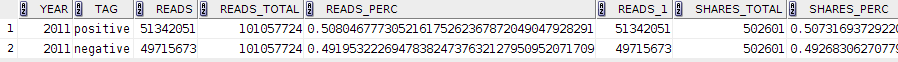
\includegraphics[scale=0.5]{art_7}
\item   Top 100 tags by article count in Business category in 2011?
\begin{lstlisting}[language=sql] 
select rank() over (order by count(a.keyarticle) desc) rank, 
 t.tag, count(a.keyarticle) articles
from oplatek.artpop_articlepopularity f
join oplatek.artpop_article a 
 on f.keyarticle = a.keyarticle 
 and a.category = 'Business' and a.publicationyear = 2011
join oplatek.artpop_tag t on 1=1
join oplatek.artpop_articletags artt 
 on a.keyarticle = artt.keyarticle and artt.keytag = t.keytag
group by t.tag
order by rank, tag asc;
\end{lstlisting}
\end{enumerate}
% subsection Article  queries (end)
     0.797 s\\ \\
      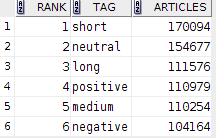
\includegraphics[scale=0.5]{art_8}
\subsection*{Advertisement  queries} % (fold)
\label{sub:Advertisement queries}

\begin{enumerate}
\item Revenue by year together with average revenue in all years together with revenue in this year and together with last year?
\begin{lstlisting}[language=sql] 
select ad.Year, sum(aa.revenue), 
  avg(sum(aa.revenue)) over () as total_avg,
  sum(sum(aa.revenue)) over 
    (order by ad.year rows 1 preceding) as sum_last_2_years
from   
advert_advertisement aa
join advert_date ad on aa.keydate = ad.keydate
group by ad.YEAR;
\end{lstlisting}
     0.155 s\\ \\
      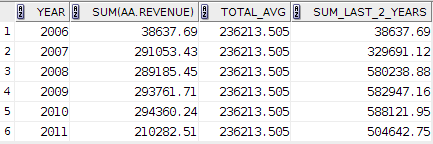
\includegraphics[scale=0.5]{adv_1}
\item    CPM(Clicks divided by displays) for top 10 advertisers by revenue together with avg CPM for advertisers category having the advertiser at least 15 campaigns?
\begin{lstlisting}[language=sql] 
select *
from 
( select
     rank() over (order by sum (aa.revenue) desc) as top,
     sum(aa.clicks)/sum(aa.displays),ac.advertiserName,
     ac.advertiserCategory as cat, 
     avg(sum(aa.clicks)/sum(aa.displays)) 
      over (partition by ac.advertiserCategory)
  from advert_advertisement aa
  join advert_campaign ac on aa.keycampaign = ac.keycampaign
  join
  ( select distinct in_aa.advertiserName 
    from advert_campaign in_aa
    group by in_aa.advertiserName
    having COUNT(in_aa.name) >= 15
  )
  camp on ac.advertiserName = camp.advertiserName
  group by rollup (ac.advertiserName,ac.advertiserCategory) 
  having grouping_id(ac.advertiserName,ac.advertiserCategory)=0
  )
where 
top < 10;
\end{lstlisting}
     0.643 s\\ \\
      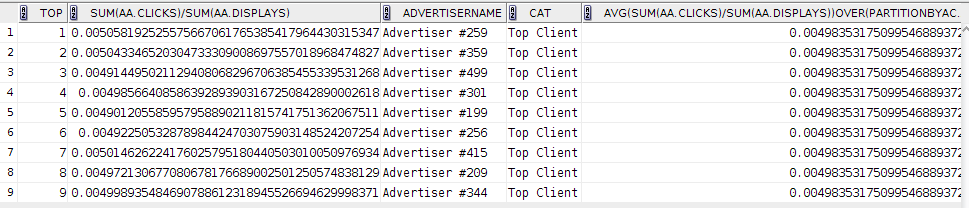
\includegraphics[scale=0.5]{adv_2}
\item Revenue by advertiser from "Small Fish" category who has greater revenue than average of the "Middle Fish" bias=0.5 together with average of "Middle Fish" advertisers? 
  \begin{lstlisting}[language=sql] 
select ac.advertiserName, ac.advertiserCategory, sum(aa.revenue), 
 avg(sum(aa.revenue)) over (partition by ac.advertiserCategory) 
 as small_fish_avg,
 ( 
  select distinct
   AVG(sum(aaa.revenue)) over 
    (partition by aac.advertiserCategory) as middle_fish_avg
    from advert_advertisement aaa 
    join advert_campaign aac on aaa.keycampaign=aac.keycampaign
    where aac.advertiserCategory = 'Medium Fish'   
    group by aac.advertiserName,aac.advertiserCategory
  ) as middle_fish_avg
from advert_advertisement aa
join advert_campaign ac on aa.keycampaign = ac.keycampaign
where ac.advertiserCategory = 'Small Fish'
group by ac.advertiserName,ac.advertiserCategory
having sum(aa.revenue) > 0.5* (
  -- having is stupid, I have to repeat query:)
  select distinct
    AVG(sum(aaa.revenue)) 
      over (partition by aac.advertiserCategory) 
    as middle_fish_avg
  from advert_advertisement aaa 
  join advert_campaign aac on aaa.keycampaign = aac.keycampaign
  where aac.advertiserCategory = 'Medium Fish'   
  group by aac.advertiserName,aac.advertiserCategory);
  \end{lstlisting}
      0.301s\\ \\
      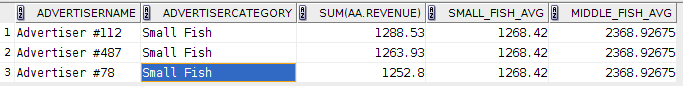
\includegraphics[scale=0.5]{adv_3}
\item    The Campaigns which lasted more than 5 month with revenue bigger than 140 at least in one from the 5 month, all in year 2011?
  \begin{lstlisting}[language=sql] 
select * from (
  select ac.name, max(sum(aa.revenue)) 
    over (partition by ac.name) as max_revenue_over_month
  from advert_advertisement aa
  join advert_date ad on ad.keyDate = aa.keyDate
  join advert_campaign ac on ac.keyCampaign = aa.keyCampaign
  where ad.year=2011
  group by ac.name, ad.month
  having ( max(ad.month) - min(ad.month)) >= 0 
    or ( (max(ad.month) - min(ad.month)) = 5 
    and (max(ad.day) - min(ad.day)) >=0 )
) where max_revenue_over_month > 140;
  \end{lstlisting}
     0.16 s\\ \\
      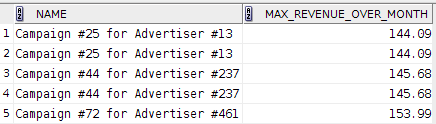
\includegraphics[scale=0.5]{adv_4}
\item Most popular campaigns by year together with their popularity(clicks+displays) and  avg CPM per month?
  \begin{lstlisting}[language=sql] 
select y, c, n, popularity, cpm_per_month
from (
  select ad.year y, ac.name n, ad.month, ac.advertisercategory c
  , sum(aa.clicks+aa.displays) popularity
  ,(avg(sum(aa.clicks)/sum(aa.displays)) 
    over (partition by ad.month order by ad.month 
    rows between 1 preceding and 1 following)) cpm_per_month
  from advert_advertisement aa
  join advert_date ad on ad.keyDate = aa.keyDate
  join advert_campaign ac on ac.keyCampaign = aa.keyCampaign
  group by ad.month,ad.year, ac.name,ac.advertisercategory
  )
order by y desc, c, popularity desc, n;
  \end{lstlisting}
     0.61 s, 35889 rows\\ \\
      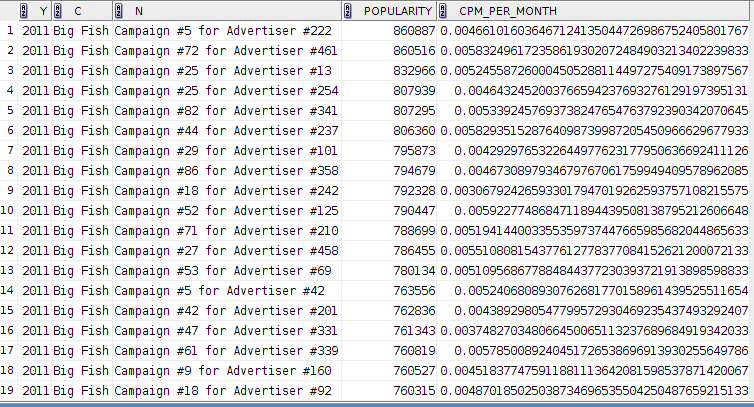
\includegraphics[scale=0.5]{adv_5}
\end{enumerate}
% section Business queries (end)

% section Advertisement business queries (end)


